\documentclass[11pt, a4paper, spanish, openright, twoside]{book}
\usepackage[spanish, activeacute]{babel}
\usepackage[utf8]{inputenc}
%\usepackage[top=2.5cm, bottom=2.5cm, outer=1.75cm, inner=1.75cm, heightrounded, marginparwidth=2.5cm, marginparsep=0.3cm]{geometry}	%márgenes empequeñecidos
\usepackage[top=2.95cm, bottom=2.25cm, outer=2.75cm, inner=2.75cm, heightrounded, marginparwidth=2.5cm, marginparsep=0.3cm]{geometry}	%márgenes originalmente
\usepackage{dpg}
\usepackage{fli}

\usepackage{pgf}
\usepackage{tikz}

\usepgflibrary{shapes.geometric} % LATEX and plain TEX and pure pgf
\usetikzlibrary{arrows,automata,positioning}
\tikzstyle{accepting by double}= [double distance=1.6pt,double,outer sep=.5\pgflinewidth+.8pt] % esto es algo estético.
\renewcommand\shorthandsspanish{}  % para compatibilizar spanish con tikz

%%%%%%		Figuras		%%%%%%%%%%%%%%%%%%%
\usepackage[vflt]{floatflt}		%Entorno float-figure

%%%%%%		Page style		%%%%%%%%%%%%%%%%%%%
\renewcommand{\thepage}{\arabic{page}}% Arabic page numbers\fancyhead{}
\pagestyle{fancy}
\fancyfoot{}
\fancyhead[LO,RE]{Ejercicio opcional 1}	%encabezado de pares: nombre de la sección
\fancyfoot[LE,RO]{\thepage}	%abajo a izqda en pares, derecha en impares: numero de pagina
%\fancyhead[LE]{\nouppercase{\leftmark}} %cuadro izquierdo de pagina par: parte y contador
\fancyfoot[CE]{Inteligencia Artificial} 
\fancyfoot[CO]{Doble Grado Informática-Matemáticas - Universidad Complutense}
\renewcommand{\footrulewidth}{0.4pt}
\renewcommand{\headrulewidth}{0.4pt}		% linea por debajo del encabezado
\renewcommand{\sectionmark}[1]{\markright{\textbf{\thesection. #1}}}	%negrita
\renewcommand{\labelitemi}{$\circ$} %Primer itemize con circunferencia vacia
\renewcommand{\labelitemii}{} %Segundo itemize con punto pequeño \cdot
\renewcommand*{\thesection}{\arabic{section}}	% Hace que no apareca el indice de capitulos y que comience en section

%%%%%%		Others		%%%%%%%%%%%%%%%%%%%
\setlength{\leftmarginii}{0em} %Segundo itemize sin sangria
\setlength{\leftmarginiii}{1em} %Tercer itemize casi sin sangria
\renewcommand{\labelitemiii}{ }
\pagenumbering{roman}
\addto{\captionsspanish}{\renewcommand*{\contentsname}{Índice}} %Cambia "Indice general" por "Indice"



\begin{document} 
\title{\Huge{\textsc{Inteligencia Artificial}} \\
	\vspace{0.7cm}
	 \textsc{\Large{Ejercicio opcional 1}} \\
	\vspace{1.5cm}
	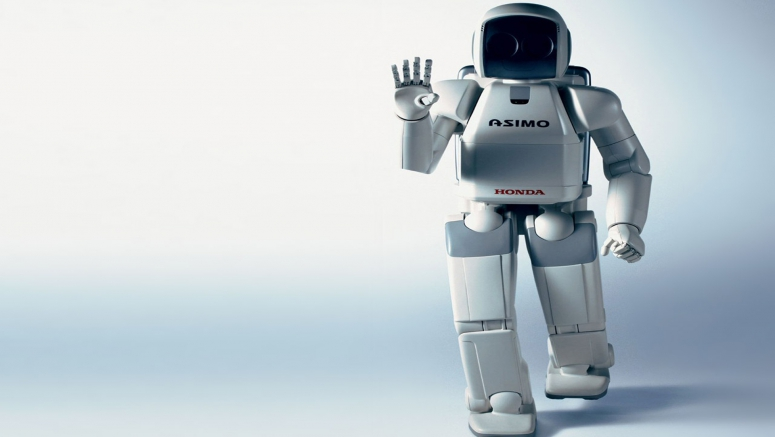
\includegraphics[scale=0.45]{robotHonda}}
\author{Enrique Ballesteros Horcajo\\
	Ignacio Iker Prado Rujas}
\date{12 de Noviembre de 2014}
\maketitle

\newpage
\mbox{}
\thispagestyle{empty}						% Hoja en blanco, sin numeros ni nada
\newpage


\tableofcontents 							%INDICE hipervinculado

\newpage
\mbox{}
\thispagestyle{empty}						% Hoja en blanco, sin numeros ni nada
\newpage

\pagenumbering{arabic}						% Pone el contador de paginas a 1 y ahora en numeros normales

\vspace{3cm}


\newpage



\begin{section}{Problema del test chino}

\textit{\textbf{Dado el problema del test chino, descrito en la transparencia 21 del tema 2.1, represéntalo como espacio de estados. Para ello, indica cómo representarás un estado, cuáles son los estados inicial y final, los operadores disponibles (sin especificar precondiciones ni poscondiciones) y su coste.}}

\textit{\textbf{Define formalmente las distintas condiciones que hacen que un estado sea peligroso y representa los 4 primeros niveles del espacio de estados sin incluir los estados peligrosos.}}


Los elementos a tener en cuenta son:

\begin{itemize}

	\item Un policía.

	\item Un ladrón.
	
	\item Dos niñas.
	
	\item Una madre.

	\item Dos niños.
	
	\item Un padre. 
	
	\item Una balsa (para dos).

\end{itemize}

Lo importante es en qué lado de la orilla se encuentran los actores, luego definimos el estado en función de eso. El estado es una 7-tupla, donde el dominio es el conjunto $\{0,1,2\}$:

$$\boxed{(policia, ladron, NNO, padre, NNA, madre, balsa)}$$

NNO es el número de niños en a orilla izquierda del río, mientras que NNA es el número de niñas en la orilla izquierda del río. En cuanto al resto de elementos:

\begin{itemize}

	\item \textbf{0 en la entrada $i-$ésima}: El elemento $i$-ésimo se encuentra en la orilla derecha (orilla objetivo). 

	\item \textbf{1 en la entrada $i-$ésima}: El elemento $i$-ésimo se encuentra en la orilla izquierda (orilla inicial).

	\item \textbf{2 en la entrada $i-$ésima}: Sólo permitido en las entradas de la tupla correspondientes a $NNO$ y $NNA$. Significa que hay dos niños/as en la orilla inicial.

\end{itemize}

En cuanto a los operadores, son 11 y suponemos que cada viaje de la balsa cuesta 1:

\begin{itemize}

	\item \texttt{cruzaP}: El policía cruza en la balsa.

	\item \texttt{cruzaPL}: El policía y el ladrón cruzan en la balsa

	\item \texttt{cruzaPA}: El padre cruza en la balsa.
	
	\item \texttt{cruzaPANO}: El padre y un niño cruzan en la balsa.
	
	\item \texttt{cruzaM}: La madre cruza en la balsa.
	
	\item \texttt{cruzaMNA}: La madre y una niña cruzan en la balsa.
	
	\item \texttt{cruzaPAM}: El padre y la madre cruzan en la balsa.
	
	\item \texttt{cruzaPNO}: El policía y un niño cruzan en la balsa.
	
	\item \texttt{cruzaPNA}: El policía y una niña cruzan en la balsa.
	
	\item \texttt{cruzaPPA}: El policía y el padre cruzan en la balsa.
	
	\item \texttt{cruzaPM}: El policía y la madre cruzan en la balsa.

\end{itemize}

	
	Peligros:
	\begin{itemize}
		\item El ladrón está sin el policía: solo es peligroso si hay alguien con él:
			\begin{itemize}
			\item El ladrón está en el lado derecho:
			
				(policia $>$ ladron)$\land$((NNO $<$ 2) $\lor$ (NNA $<$ 2) $\lor$ (padre $<$ 1) $\lor$ (madre $<$ 1))
				
			\item El ladrón está en el lado izquierdo:
			
				(policia $<$ ladron)$\land$((NNO $>$ 0) $\lor$ (NNA $>$ 0) $\lor$ (padre $>$ 0) $\lor$ (madre $>$ 0))
		\end{itemize}
		
		\item El padre está con alguna niña y la madre no está, o la madre está con algún niño y el padre no está:
			
				(padre $>$ madre)$\land$((NNO $<$ 2) $\lor$ (NNA $>$ 0) )
			
				(padre $<$ madre)$\land$((NNO $>$ 0) $\lor$ (NNA $<$ 2) )
	
		
	
	\end{itemize}

	Árbol de estados no peligrosos:
\begin{center}
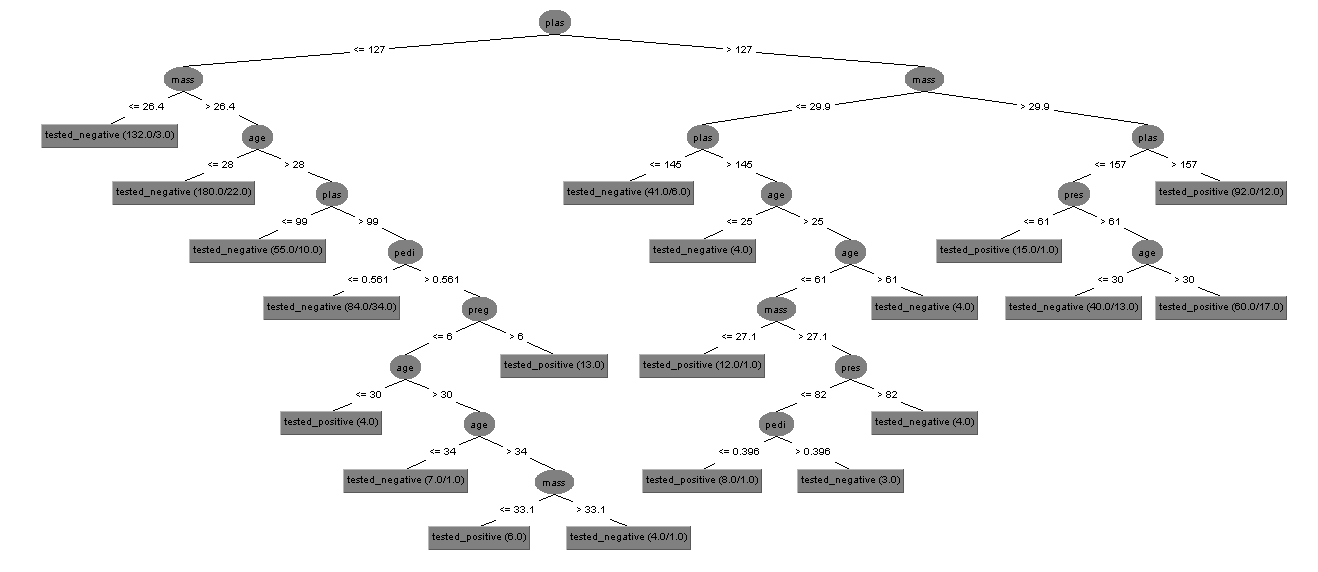
\includegraphics[scale=0.65]{arbol.png}
\end{center}
	
\begin{thebibliography}{9}

\bibitem{aima}
	Russell, S.; Norvig, P, \\
	\emph{Artificial Intelligence, a modern aproach}.\\
	New Jersey: Pearson, 2010.
	
\bibitem{clase}
	Apuntes y transparencias de Inteligencia Artificial, \\
	Doble Grado Matemáticas - Ing. Informática, U.C.M., 2014-2015.

\end{thebibliography}
\end{section}

\end{document}

